\documentclass[10pt]{beamer}
\usetheme[
%%% option passed to the outer theme
%    progressstyle=fixedCircCnt,   % fixedCircCnt, movingCircCnt (moving is deault)
  ]{Feather}
  
% If you want to change the colors of the various elements in the theme, edit and uncomment the following lines

% Change the bar colors:
\setbeamercolor{Feather}{fg=black!20,bg=black}

% Change the color of the structural elements:
\setbeamercolor{structure}{fg=black}

% Change the frame title text color:
%\setbeamercolor{frametitle}{fg=blue}

% Change the normal text color background:
%\setbeamercolor{normal text}{fg=black,bg=gray!10}

%-------------------------------------------------------
% INCLUDE PACKAGES
%-------------------------------------------------------

\usepackage[utf8]{inputenc}
\usepackage[english]{babel}
\usepackage[T1]{fontenc}
\usepackage{graphicx}
\usetheme{Warsaw}
\usepackage[texcoord,
grid,
gridunit=mm,
gridcolor=red!60,
subgridcolor=black!60]{eso-pic}
\usepackage[absolute,overlay]{textpos}
\usepackage{pgf,pgfarrows,pgfnodes,pgfautomata,pgfheaps,pgfshade}
\usepackage{listings}
\usepackage{pgfplots}
\usepackage{tcolorbox}
\usepackage{bibunits}
\usepackage{amsmath,amsthm,amssymb}
%-------------------------------------------------------
% DEFFINING AND REDEFINING COMMANDS
%-------------------------------------------------------

% colored hyperlinks
\newcommand{\chref}[2]{
  \href{#1}{{\usebeamercolor[bg]{Feather}#2}}
}
%%%%%%%%%%%%%%%%%%%%%%%%%%%%%%%%%%%%%%%%%%%%%%%%%%%%%%%%%%%%%
\mode<presentation>
{  
	%\usetheme{PaloAlto}
	%\usecolortheme[named=kugreen]{structure}
	\useinnertheme{progressbar}
	%\usefonttheme{default}
	%\usefonttheme{serif}
	%\setbeamercovered{transparent}
	%\setbeamertemplate{blocks}[rounded][shadow=true]
	%s\setbeamertemplate{navigation symbols}[only frame symbol]
}

%-------------------------------------------------------
% INFORMATION IN THE TITLE PAGE
%-------------------------------------------------------
\defaultbibliography{tomato_control}

\title[] % [] is optional - is placed on the bottom of the sidebar on every slide
{ % is placed on the title page
      \textbf{Modeling of optimal phytosanitary policies in crops of economic importance in the state of Sonora.}
}

\subtitle[Doctorado en Ciencias Matem\'aticas]
{
      \textbf{}
}

\author[Gabriel Adri\'an Salcedo Varela]
{      Gabriel Adri\'an Salcedo Varela
}

\institute[]
{
      Departamento de matem\'aticas, Divisi\'on de Ciencas Exactas y Naturales\\
    Universidad de Sonora\\
  
  %there must be an empty line above this line - otherwise some unwanted space is added between the university and the country (I do not know why;( )
}

\date{\today}

%-------------------------------------------------------
% THE BODY OF THE PRESENTATION
%-------------------------------------------------------
%%%%%%%%%%%%%%%%%%%%%%%%%%%%%%%%%%%%%%%%%%%%%%%%%%%%%%%%%%%%%%%%%%%%%%%%%%%%%%%%
\def\Q#1#2{\frac{\partial #1}{\partial #2}}
\usetikzlibrary{arrows,shapes}
%\pgfplotsset{compat=1.14}
%%%%%%%%%%%%%%%%%%%%%%%%%%%%%%%%%%%%%%%%%%%%%%%%%%%%%%%%%%%%%%%%%%%%%%%%%%%%%%%%
%-----------------------------ExtrasDeTercerPresentacion
%--------------------------------Fancyboxes-------------------------------------
\definecolor{myblue}{rgb}{.8, .8, 1}
\definecolor{azure(colorwheel)}{rgb}{0.0, 0.5, 1.0}
\definecolor{shadecolor}{cmyk}{0,0,0.41,0}
\newcommand*\mybluebox[1]{%
    \colorbox{myblue}{\hspace{1em}#1\hspace{1em}}
}
\newcommand*\myyellowbox[1]{%
    \colorbox{darkyellow}{\hspace{1em}#1\hspace{1em}}
}
%--------------------------------------------------------------------------
\definecolor{shadecolor}{cmyk}{0,0,0.41,0}
\definecolor{light-blue}{cmyk}{0.25,0,0,0}
\newsavebox{\mysaveboxM} % M for math
\newsavebox{\mysaveboxT} % T for text
\newcommand*\Garybox[2][Example]{%
    \sbox{\mysaveboxM}{#2}%
        \sbox{\mysaveboxT}{\fcolorbox{black}{light-blue}{#1}}%
            \sbox{\mysaveboxM}{%
    \parbox[b][\ht\mysaveboxM+.5\ht\mysaveboxT+.5\dp\mysaveboxT][b]{%
        \wd\mysaveboxM}{#2}%
    }%
    \sbox{\mysaveboxM}{%
        \fcolorbox{black}{shadecolor}{%
        \makebox[\linewidth-10em]{\usebox{\mysaveboxM}}%
        }%
    }%
    \usebox{\mysaveboxM}%
    \makebox[0pt][r]{%
        \makebox[\wd\mysaveboxM][c]{%
            \raisebox{\ht\mysaveboxM-0.5\ht\mysaveboxT
            +0.5\dp\mysaveboxT-0.5\fboxrule}{\usebox{\mysaveboxT}}%
        }%
    }%
}
\newcommand\Fontvi{\fontsize{7}{7.2}\selectfont}
%%%%%%%%%%%%%%%%%%%%%%%%%%%%%%%%%%%%%%%%%%%%
\definecolor{kugreen}{RGB}{50,93,61}
\definecolor{kugreenlys}{RGB}{132,158,139}
\definecolor{kugreenlyslys}{RGB}{173,190,177}
\definecolor{kugreenlyslyslys}{RGB}{214,223,216}
\definecolor{greenArea}{RGB}{124,252,124}
\definecolor{hellmagenta}{rgb}{1,0.75,0.9}
\definecolor{hellcyan}{rgb}{0.75,1,0.9}
\definecolor{hellgelb}{rgb}{1,1,0.8}
\definecolor{colKeys}{rgb}{0,0,1}
\definecolor{colIdentifier}{rgb}{0,0,0}
\definecolor{colComments}{rgb}{1,0,0}
\definecolor{colString}{rgb}{0,0.5,0}
\definecolor{darkyellow}{rgb}{1,0.9,0}
\setbeamercovered{transparent}
\lstset{%
    language=[AlLaTeX]TEX,%
    float=hbp,%
    basicstyle=\ttfamily\small, %\usepackage{cir}
    identifierstyle=\color{colIdentifier}, %
    keywordstyle=\color{colKeys}, %
    stringstyle=\color{colString}, %
    commentstyle=\color{colComments}, %
    columns=flexible, %
    tabsize=3, %
    frame=single, %
    extendedchars=true, %
    showspaces=false, %
    showstringspaces=false, %
    numbers=left, %
    numberstyle=\tiny, %
    breaklines=true, %
    backgroundcolor=\color{hellgelb}, %
    breakautoindent=true, %
    captionpos=b,%
    xleftmargin=18pt,%
    xrightmargin=\fboxsep%
}
\pgfplotsset{
    left segments/.code={\pgfmathsetmacro\leftsegments{#1}},
    left segments=3,
    left/.style args={#1:#2}{
        ybar interval,
        domain=#1:#2,
        samples=\leftsegments+1,
        x filter/.code=\pgfmathparse{\pgfmathresult}
       }
}
\DeclareMathOperator{\sign}{sgn}
\newcommand{\innerprod}[2]{\left\langle#1, #2\right\rangle}
\newcommand\bound{10} % bound number of points on each side of N
\newcommand\labelnum[3][]{
    \begin{scope}[font=\footnotesize,x=.3cm,#1]
      \foreach \mypt in {0,#2,...,\bound}{
        \draw(\mypt,0)circle[radius=2pt];
        \draw(-\mypt,0)circle[radius=2pt];
      }
      \draw(-\bound-5,0)--(\bound+5,0) node[pos=0, left]{$t$};
      \node(start)[at={(-\bound-4,0)},label=below:{$t_0=0$}]{$[$};
      \node(end)[at={(\bound+4,0)},label=below:{$T=Nh$}]{$]$};
      \node[%
          at={($(start)!.319!(end)$)},
          label=below:{
               $\underbrace{}_{h}$
            }%
            ]{\vphantom{$[$}};
      \node[at={($(start)!.57!(end)$)},label=below:{$t_{n+1}$}]{\vphantom{$[$}};
      \filldraw(0,0)circle[radius=2pt];
      \node[at={(-\bound-2,0)},above]{$\cdots$};
      \node[at={(\bound+2,0)},above]{$\cdots$};
      \node[at={(0,0)},above=5pt]{#3};
    \end{scope}
}
\usepackage{remreset}
\makeatletter
\@removefromreset{subsection}{section}
\makeatother
\definecolor{greenstrong}{rgb}{0.58,0.77,0.29}
\definecolor{redstrong}{rgb}{0.81,0.22,0.23}
\definecolor{fglisting}{gray}{0.3}
\definecolor{bglisting}{gray}{1}
\definecolor{fgshell}{gray}{1}
\definecolor{bgshell}{gray}{0.1}
\definecolor{bgshelllight}{gray}{0.8}
\definecolor{cadmiumorange}{rgb}{0.93, 0.53, 0.18}
\definecolor{byzantium}{rgb}{0.44, 0.16, 0.39}
\definecolor{capri}{rgb}{0.0, 0.75, 1.0}
%


\setcounter{subsection}{1}
\newcommand{\hl}[1]{\textbf{\textcolor{greenstrong}{#1}}}
\newcommand{\hb}[1]{\textbf{\textcolor{azure(colorwheel)}{#1}}}
\newcommand{\hlErr}[1]{\textcolor{redstrong}{\texttt{#1}}}
\newcommand{\hlOk}[1]{\textcolor{green}{\texttt{#1}}}
\newcommand{\hlInv}[1]{\colorbox{bgshell}{\textcolor{fgshell}{\texttt{#1}}}}
\newcommand{\unhl}[1]{\textcolor{gray}{#1}}
\newcommand{\clda}[0]{$\textcolor{blue}{\lambda}$}
\newcommand{\carr}[0]{$\textcolor{purple}{\rightarrow}$}
\newcommand{\cbind}[0]{\textbf{\texttt{$>\!\!>\!\!=$}}}
\newcommand{\codedots}[0]{\textcolor{mid-gray}{...}}

%
\tcbuselibrary{skins, breakable}
\newtcolorbox{greenbox}[1]{%
        colback = green!5!white,
        colframe = green!55!black,
        fonttitle = \bfseries,
        title = #1 %
    }
\newtcolorbox{bluebox}[1]{%
        colback = blue!5!white,
        colframe = blue!55!black,
        fonttitle = \bfseries,
        title = #1
    }
%
\newtcolorbox{graybox}[1]{%
        colback = gray!5!white,
        colframe = gray!55!black,
        fonttitle = \bfseries,
        title = #1
    }
%
\newtcolorbox{yellowbox}[1]{%
        colback = yellow!5!white,
        colframe = yellow!55!black,
        fonttitle = \bfseries,
        title = #1
    }

\begin{document}
% Define block styles
%-------------------------------------------------------
% THE TITLEPAGE
%-------------------------------------------------------

{\1% % this is the name of the PDF file for the background
\begin{frame}[plain,noframenumbering] % the plain option removes the header from the title page, noframenumbering removes the numbering of this frame only
  \titlepage % call the title page information from above
\end{frame}}


\begin{frame}{Contents}{}
\tableofcontents
\end{frame}
%----______________________________
% [<+->]: itemize animation
%-------------------------------------------------------
%-------------------------------------------------------

\section{Motivation}

\begin{frame}
\frametitle{Tomato Leaf Curl Virus}
	\begin{textblock*}{40mm}(5mm,20mm)
		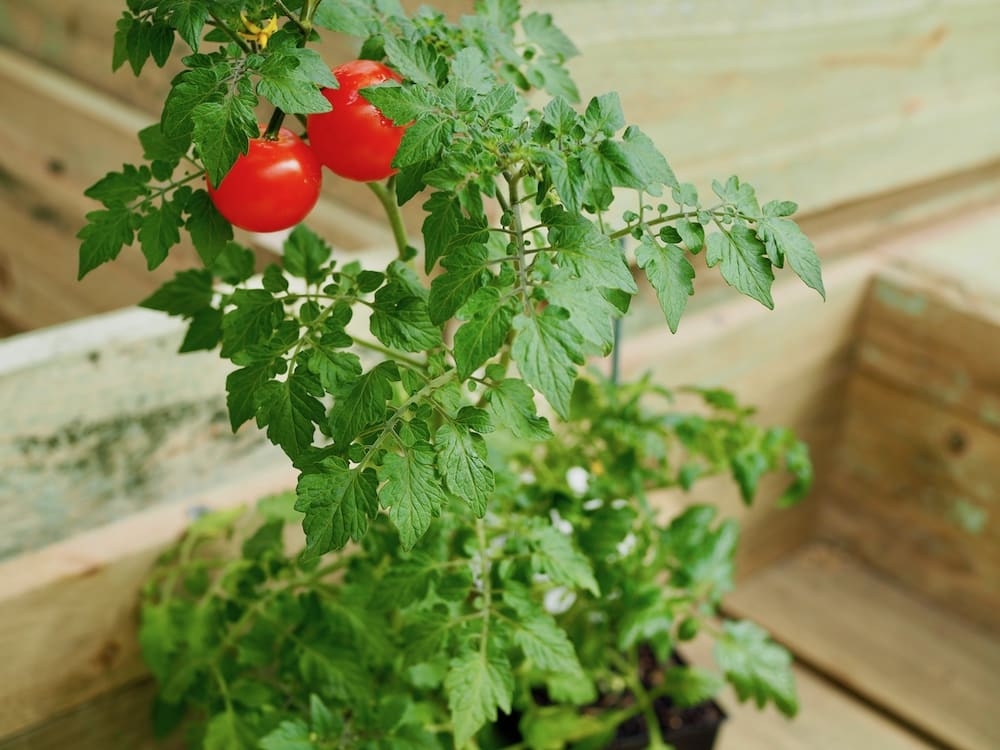
\includegraphics[width=\linewidth]{Feathergraphics/Tomato_plant.eps}
	\end{textblock*}

	\begin{textblock*}{30mm}(85mm,20mm)
		\includegraphics[width=\linewidth]{Feathergraphics/TYLCV_3_bush.eps}
	\end{textblock*}
	\begin{textblock*}{45mm}(30mm,60mm)
		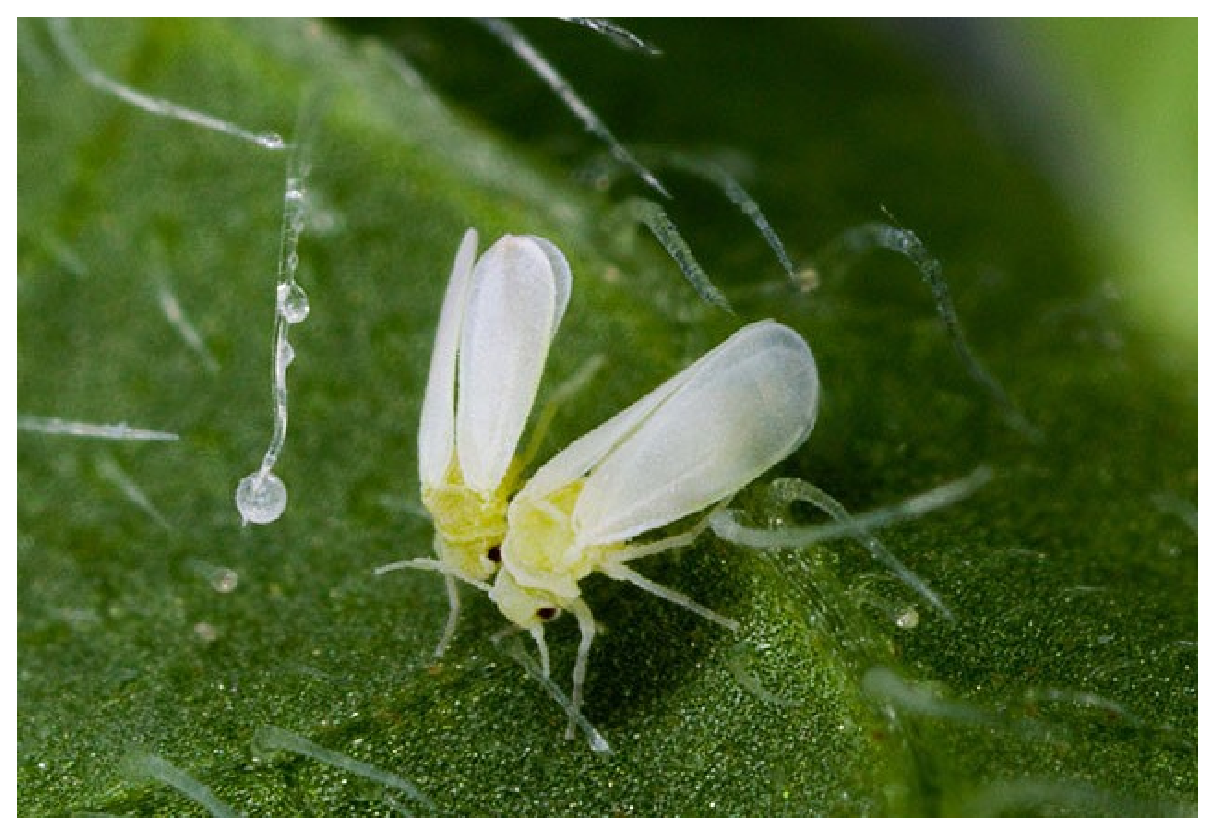
\includegraphics[width=\linewidth]{Feathergraphics/Mosca_Blanca.eps}
	\end{textblock*}
\end{frame}

\begin{frame}
	\begin{textblock*}{45mm}(10mm,25mm)
				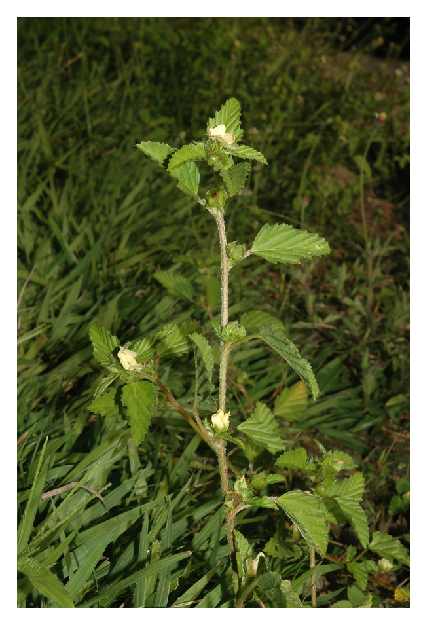
\includegraphics[width=\linewidth]{Feathergraphics/Malvastrum_coromancalianum_L.eps}
	\end{textblock*}
	\begin{textblock*}{50mm}(65mm,25mm)
				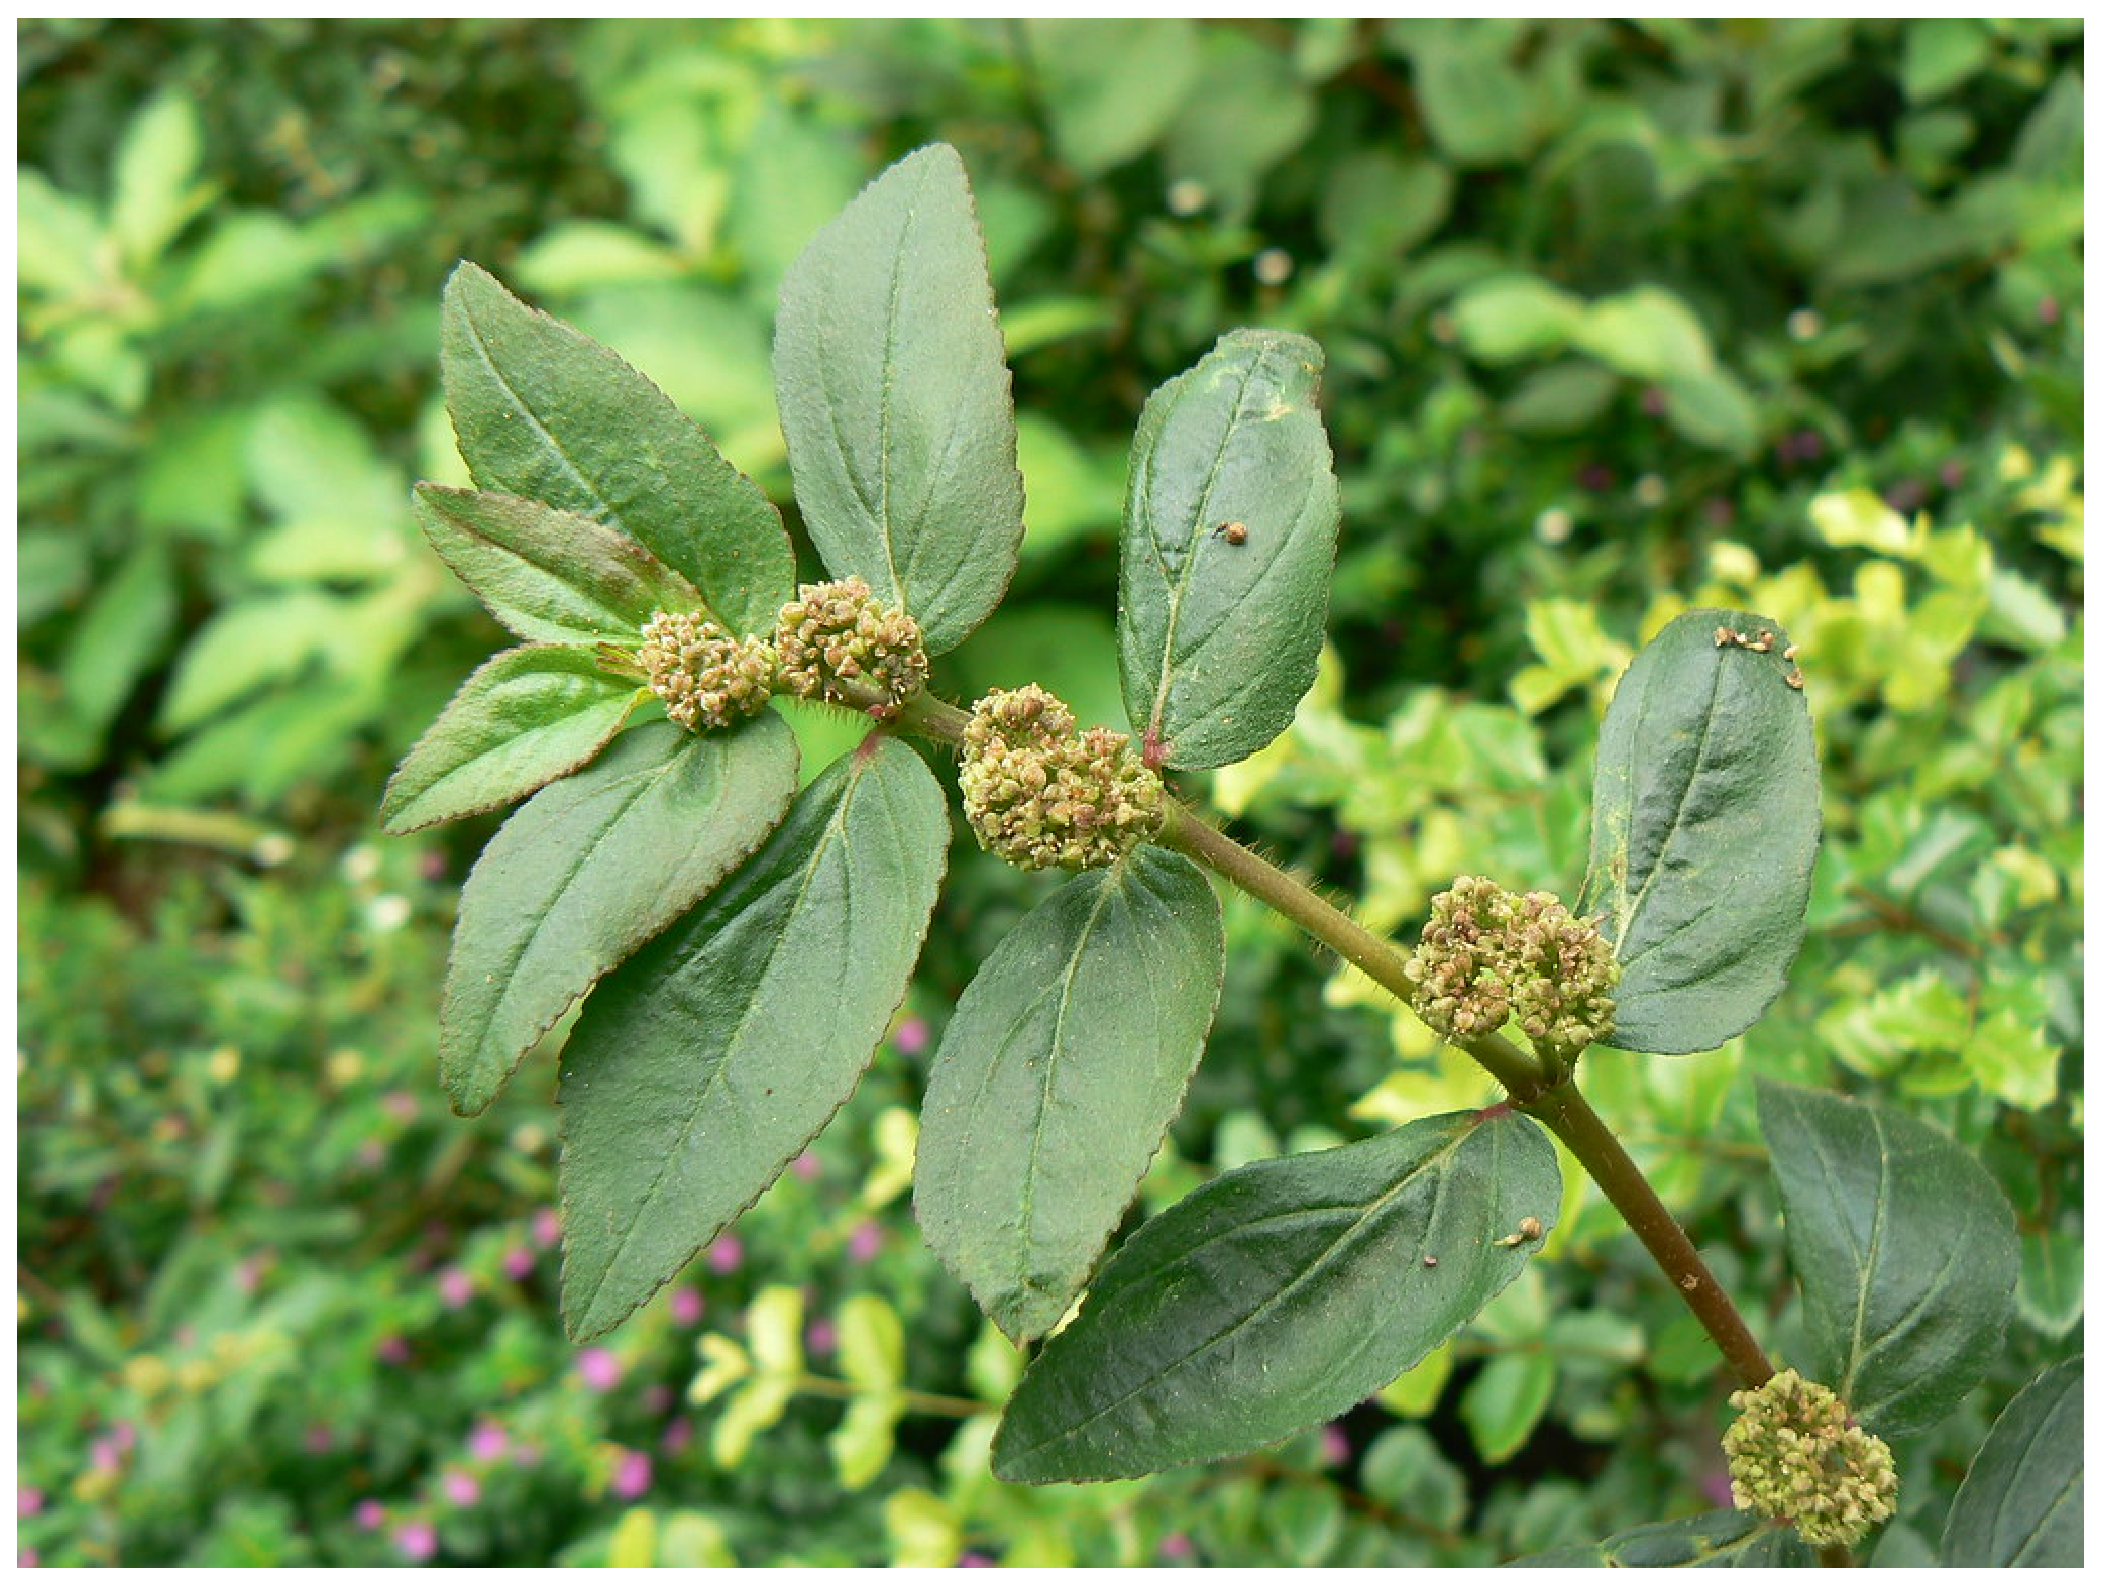
\includegraphics[width=\linewidth]{Feathergraphics/Euphorbia_geniculata_Ort.eps}
	\end{textblock*}	
\end{frame}

\section{Objetive}
\begin{frame}{}{}
	\begin{block}{Objetive}
		Model optimal phytosanitary policies for diseases in agricultural crops.
	\end{block}
	
\end{frame}

\section{Epidemical Model}

%%%%%%%%%%%%%%%%%%%%%%%%%%%%%%%%%%%%%%%%%%%%%%%%%%%%%%%%%%%%%%%%%%%%
\begin{frame}{}
\begin{bibunit}[abbrv]
	\nocite{Holt1999b}
	\putbib
\end{bibunit}
\end{frame}

%%%%%%%%%%%%%%%%%%%%%%%%%%%%%%%%%%%%%%%%%%%%%%%%%%%%%%%%%%%%%%%%%%%%%
\begin{frame}{Plant Model without control}{Tomato Leaf Curl Virus Disease Using an Epidemiological Model}
\begin{textblock*}{60mm}(65mm,25mm)
    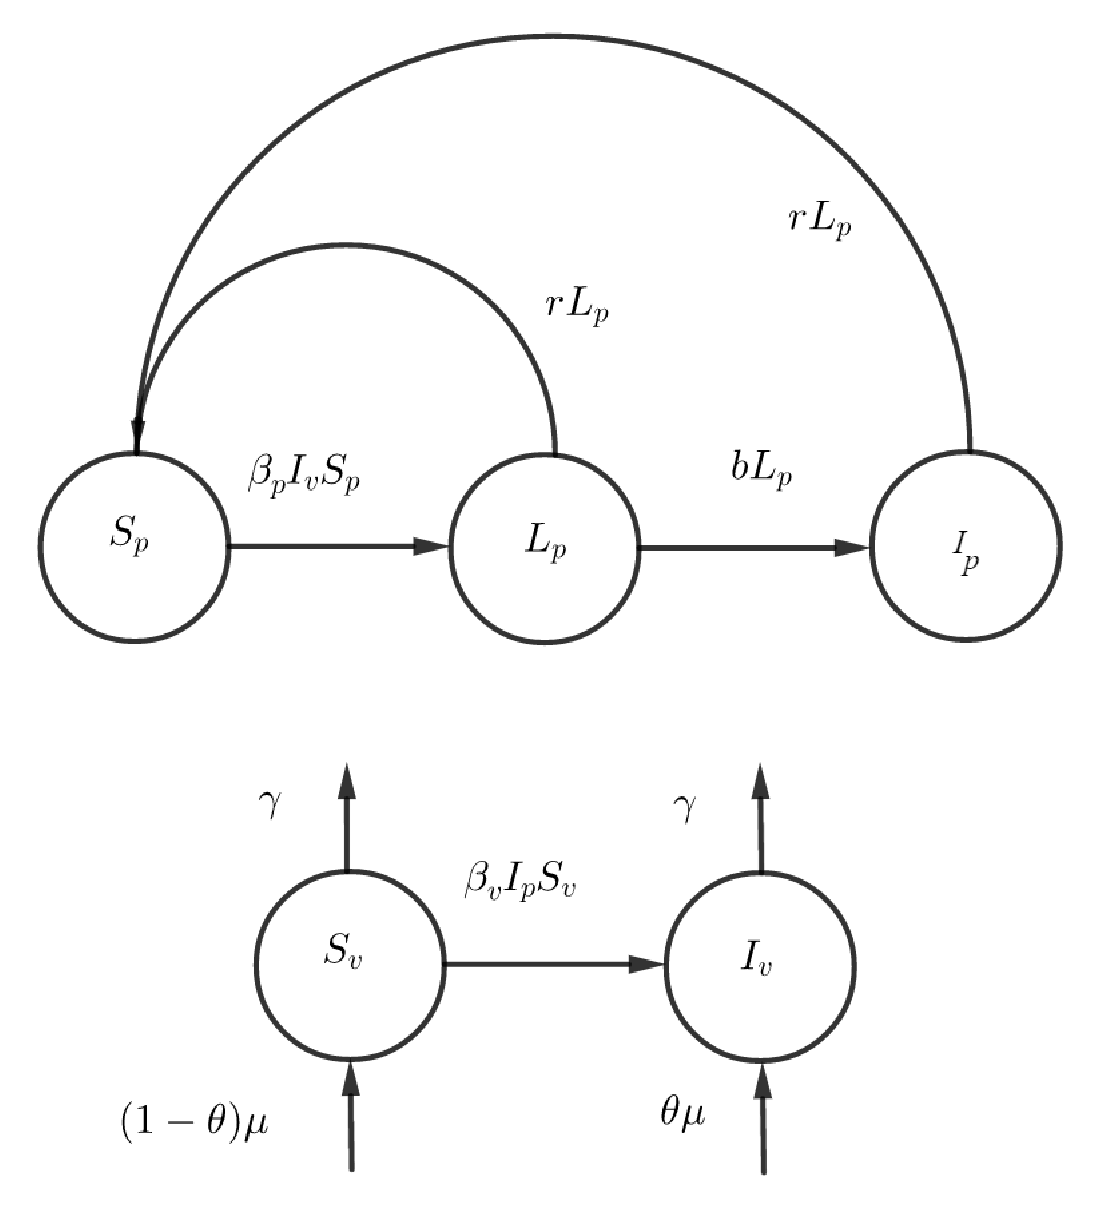
\includegraphics[width=\linewidth]{Feathergraphics/plant_diagram.eps}
\end{textblock*}
\begin{textblock*}{55mm}(5mm,25mm)
	\begin{graybox}{Hypothesis:}
		
		\begin{itemize}
			\item infection by infeted plants and vectors,
			\item output and input for plants and vectors. 
		\end{itemize}
		\end{graybox}	
\end{textblock*}
\end{frame}

\begin{frame}
\frametitle{Others Controls}
	\begin{textblock*}{40mm}(2mm,22mm)

		\begin{graybox}{Cultural Control}
			\begin{itemize}
				\item<1-> physical barriers,
				\item<2-> planting dates,
				\item<3-> removal of infested plants,
				\item<4-> host plant resistance.
			\end{itemize}
		\end{graybox}
		\end{textblock*}

	\begin{textblock*}{40mm}(43mm,22mm)
		\begin{graybox}{Biological control}
			\begin{itemize}
				\item<5-> Parasitoids,
				\item<6-> predators
				\item<7-> fungi.
			\end{itemize}
		\end{graybox}
	\end{textblock*}

	\begin{textblock*}{42mm}(85mm,22mm)
		\begin{graybox}{Insecticide}
			\begin{itemize}
				\item<8-> Pymetrozine,
				\item<9-> flupyradifurone,
				\item<10-> cyazypyr.
			\end{itemize}
		\end{graybox}
\end{textblock*}

\begin{textblock*}{90mm}(45mm,47mm)	
	\begin{bibunit}[abbrv]
		\nocite{Shun-xiang2001}
		\putbib
	\end{bibunit}
\end{textblock*}

\begin{textblock*}{120mm}(10mm,70mm)
	\begin{bibunit}[abbrv]
		\nocite{Smith2014}
		\putbib
	\end{bibunit}
\end{textblock*}

\end{frame}

\begin{frame}	
		\begin{textblock*}{62mm}(2mm,15mm)
			\begin{greenbox}{}
				\begin{align*}
            		\frac{dS_p}{dt} &=-\beta_p S_p I_v +\textcolor{capri}{r}
             			(L_p +  I_p),\\
            		\frac{dL_p}{dt} &= \beta_p S_p I_v -b L_p 
            			-\textcolor{capri}{r} L_p,\\
            		\frac{dI_p}{dt} &= b L_p - \textcolor{capri}{r} I_p,\\
           			\frac{dS_v}{dt} &=-\beta_v S_v I_p - \textcolor{cadmiumorange}{\gamma} S_v   -(1-\theta)\mu,\\
            		\frac{dI_v}{dt} &=  \beta_v S_v I_p -\textcolor{cadmiumorange}{\gamma} I_v	-\theta\mu,\\
								S_p(0) &= S_{p_0}, L_p(0) = L_{p_0}, I_p(0) = I_{p_0},\\
								S_v(0) &= S_{v_0}, I_v(0) = I_{v_0}.
				\end{align*}
			\end{greenbox}
		\end{textblock*}
	
	\begin{textblock*}{60mm}(65mm,15mm)
		\begin{tabular}{|c |c |l |} 
				\hline
				Par. & Value & Descrip. \\ [0.5ex] 
				\hline
				$\beta_p$ & 0.1 & plant latent rate  \\ 
				\hline
				$r$ & 0.01 & plant remove rate \\
				\hline
				$b$ & 0.075 & plant infectious rate\\
				\hline
				$\gamma$ & 0.06 &  vector die or depar rate \\
				\hline
				$\mu$ & 0.3 & immigration rate \\
				\hline
				$\theta$ & 0.2 & infected vectors arrival \\
				\hline
				$\beta_v$ &0.003 & vector infected rate\\ 
				\hline
	\end{tabular}
	\end{textblock*}

	\begin{textblock*}{50mm}(70mm,55mm)
    	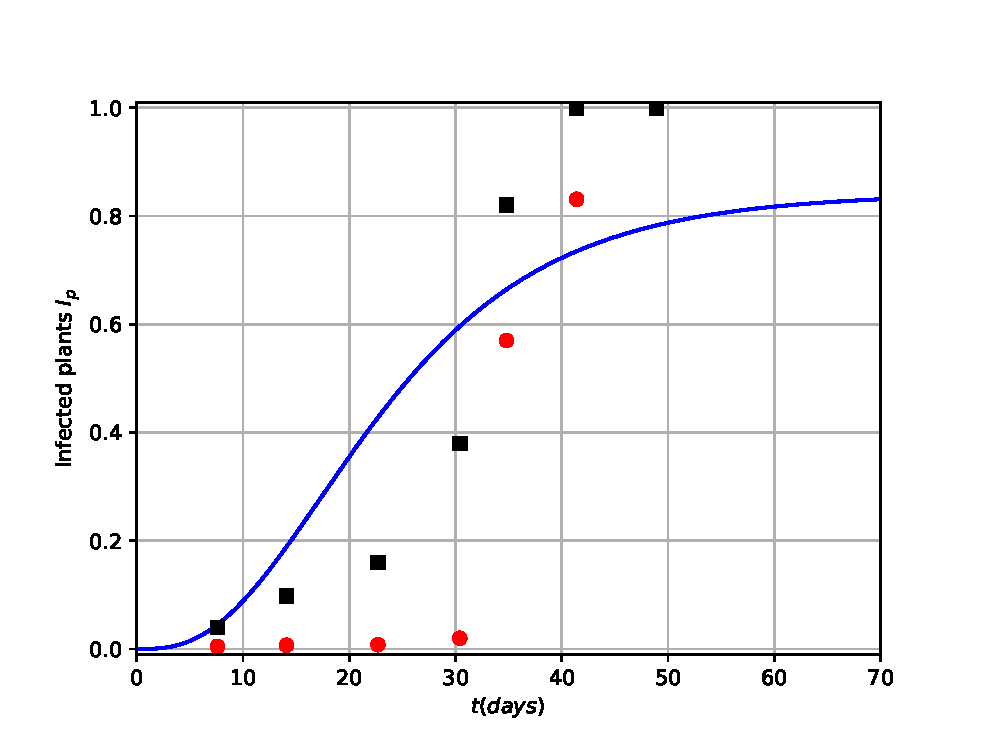
\includegraphics[width=\linewidth]{Feathergraphics/Simulation_data.eps}
	\end{textblock*}
\end{frame}
%-------------------------------------------------------------------------------
\begin{frame}
	\begin{textblock*}{50mm}(5mm,15mm)
		\begin{greenbox}{}
			\begin{equation*}
				R_0=\sqrt{\frac{\beta_v\mu b\beta_p}{r^2(r+b)\gamma}}.
			\end{equation*}
		\end{greenbox}
	
	\begin{textblock*}{70mm}(5mm,45mm)
		\begin{yellowbox}{}
			If $R_0<1,$
			\begin{equation*}
			\lim\limits_{t\rightarrow \infty}(S_p,L_p,I_p,S_v,I_v)=(N_p,0,0,\frac{\mu}{\gamma},0).
			\end{equation*}
				If $R_0<1,$
			\begin{equation*}
			\lim\limits_{t\rightarrow \infty}(S_p,L_p,I_p,S_v,I_v)=(S_p^*,L_p^*,I_p^*,S_v^*,I_v^*).
			\end{equation*}
		\end{yellowbox}
	\end{textblock*}
	
		
	\end{textblock*}
	\begin{textblock*}{50mm}(77mm,15mm)
		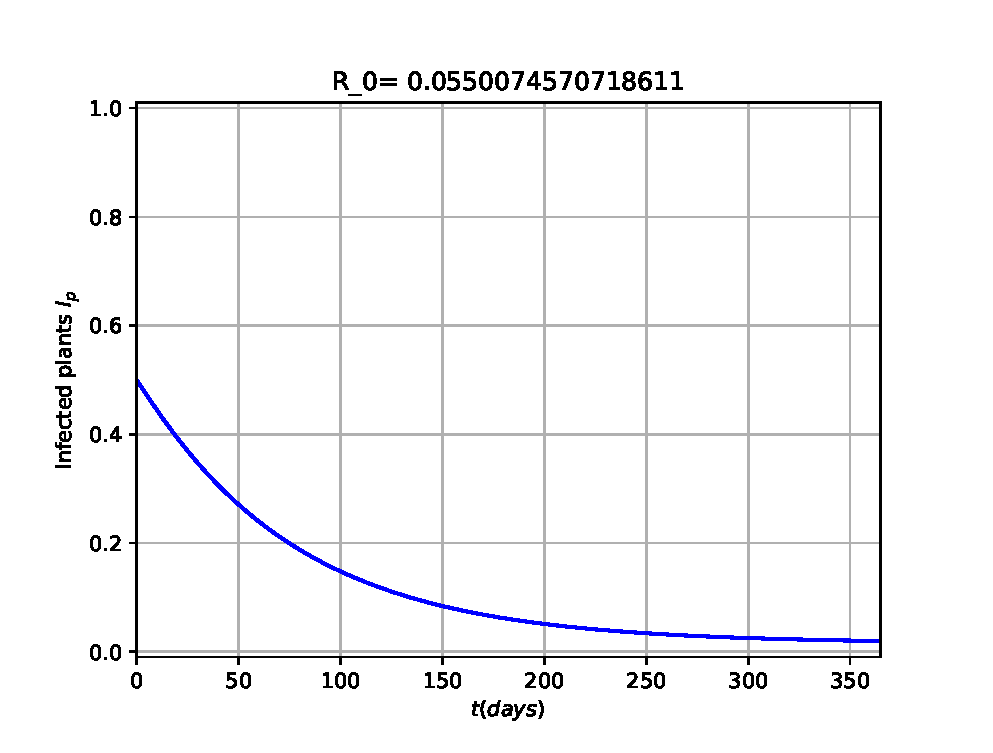
\includegraphics[width=\linewidth]{Feathergraphics/Tomato_simulation_1.eps}
		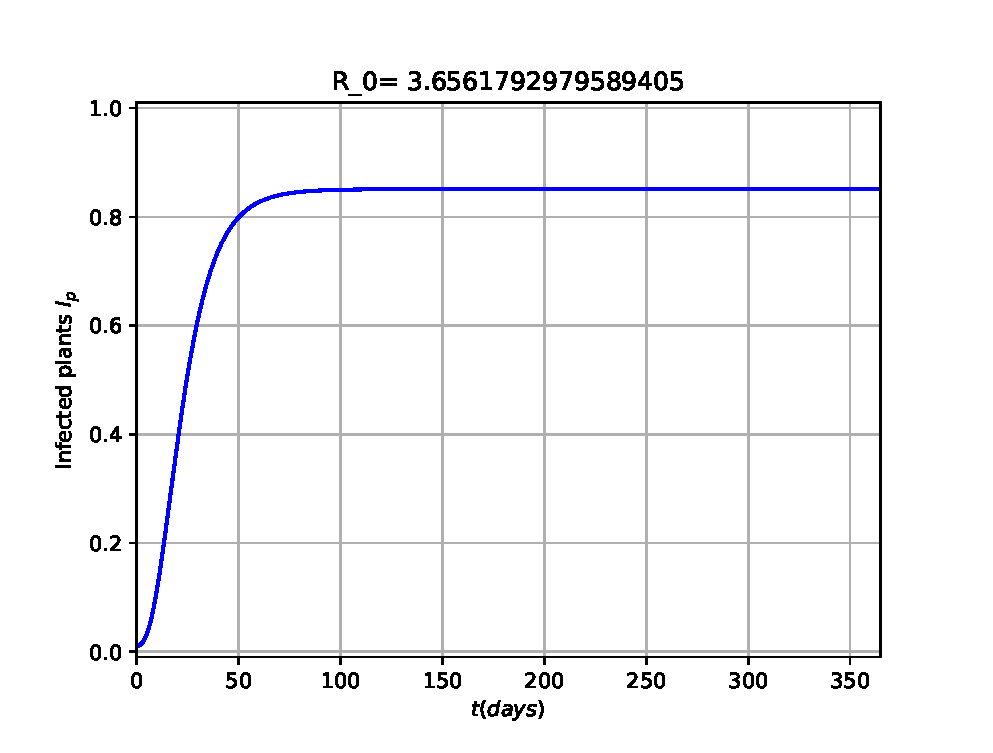
\includegraphics[width=\linewidth]{Feathergraphics/Tomato_simulation_2.eps}
	\end{textblock*}	
\end{frame}
%%-------------------------------------------------------
%%-------------------------------------------------------
%
%%-------------------------------------------------------
%-------------------------------------------------------
\subsection{Controlled Model}
\begin{frame}{Plant Model with control}{Tomato Leaf Curl Virus Disease Using an Epidemiological Model}

        \begin{align*}
            \frac{dS_p}{dt} &=-\beta_p S_p I_v +(r +u_1)L_p + (r + u_2) I_p,\\
            \frac{dL_p}{dt} &=\beta_p S_p I_v -b L_p -(r + u_1)L_p,\\
            \frac{dI_p}{dt} &= b L_p - (r + u_2) I_p,\\
            \frac{dS_v}{dt} &=-\beta_v S_v I_p - (\gamma+u_3) S_v -(1-\theta)\mu,\\
            \frac{dI_v}{dt} &=\beta_v S_v I_p -(\gamma+u_3) I_v -\theta\mu,				
        \end{align*}
\end{frame}


\begin{frame}
	\begin{textblock*}{120mm}(2mm,12mm)
		Minimize
		\begin{align*}
			J(u_1,u_2,u_3)&=\int_{0}^T	A_1 I_p(t) + A_2 L_p(t) + A_3 I_v(t)
			+ c_1 u_1(t)^2+ c_2 u_2(t)^2\\ &+ c_3 u_3(t)^2 dt,
		\end{align*}
	\end{textblock*}
	\begin{textblock*}{20mm}(2mm,32mm)
		subject to
	\end{textblock*}

	\begin{textblock*}{120mm}(20mm,40mm)
		\hspace{50mm}	$\left\{ \begin{array}{ll}
%				\begin{align*}
				\frac{dS_p}{dt} = &-\beta_p S_p I_v +(r +u_1)L_p + (r + u_2) I_p,\\\\
				\frac{dL_p}{dt} =&\beta_p S_p I_v -b L_p -(r + u_1)L_p,\\\\
				\frac{dI_p}{dt} =& b L_p - (r + u_2) I_p,\\\\
				\frac{dS_v}{dt} =&-\beta_v S_v I_p - (\gamma+u_3) S_v -(1-\theta)\mu,\\\\
				\frac{dI_v}{dt} =&\beta_v S_v I_p -(\gamma+u_3) I_v -\theta\mu,\\\\
				S_p(0) &= S_{p_0}, L_p(0) = L_{p_0},I_p(0) = I_{p_0},S_v(0) = S_{v_0}, I_v(0) = I_{v_0}.			
%				\end{align*}
			\end{array}\right.$
	\end{textblock*}
\end{frame}

%-------------------------------------------------------
%-------------------------------------------------------
%
%% Aquí va la teoria de exitencia y pontryagain
%
%-------------------------------------------------------
%-------------------------------------------------------
\section{Existence Theory}

\begin{frame}

\begin{textblock*}{65mm}(3mm,15mm)
	\begin{greenbox}{}
		$T\in (0,\infty)$ be fixed. Consider the control system:

		$$\left\{ \begin{array}{l}
		\dot{x}(s)=f(s,u(s),x(s))\,\,s\in [t_0,T], \\
		x(t_0)=x_0,\\
		\end{array}
		\right.$$

		with terminal state constraint
		$$x(T;t_0,x_0,u(\cdot))\in M,$$
		where $M\subseteq \mathbb{R}^n$ is fixed.
	\end{greenbox}
\end{textblock*}

\begin{textblock*}{55mm}(70mm,15mm)
	\begin{yellowbox}{}
		$M:\mathbb{R}_{+}\rightarrow 2^{\mathbb{R}^n}$ is a moving target in $\mathbb{R}^n$ if for any $t\in \mathbb{R}_{+}$, $M(t)$ is a measurable.
	\end{yellowbox}
\end{textblock*}

\end{frame}


\begin{frame}
	\begin{textblock*}{120mm}(5mm,15mm)
		\begin{yellowbox}{}
			$$J(t_0,x_0;u(\cdot))=\int_{t_0}^{T}g(s,u(s),x(s))ds+h(T,x(T))\equiv J^T(t_0,x_0,u(\cdot)).$$
		\end{yellowbox}
	\end{textblock*}
	\begin{textblock*}{110mm}(10mm,40mm)
		\begin{graybox}{Problem $(OC)^T$}
			Given $(t_0,x_0)\in \mathbb{R}_{+}\times \mathbb{R}^n$ with $\tilde{\mathcal{U}}^M_{x_0}[t_0,T]\neq\emptyset$, find a $\bar{u}(\cdot)\in \tilde{\mathcal{U}}^M_{x_0}[t_0,T]$ such that
			
			\begin{equation*}
			J^T(t_0,x_0;\bar{u}(\cdot))=\inf_{u(\cdot)\in \tilde{\mathcal{U}}^M_{x_0}[t_0,T]} J^T(t_0,x_0;u(\cdot)).
			\end{equation*}
		
		\end{graybox}
	\end{textblock*}
\end{frame}

\begin{frame}
\begin{textblock*}{120mm}(5mm,15mm)
	\begin{graybox}{(C1)}
		$f:\mathbb{R}_{+}\times U\times \mathbb{R}^n\rightarrow \mathbb{R}^n$ is measurable, satisfies a lipchitz condition in $x$, and $|f(t,u,0)|\leq L,\,\mbox{for every}\,(t,u)\in \mathbb{R}_{+}\times U .$
				
	\end{graybox}
\end{textblock*}

\begin{textblock*}{120mm}(5mm,40mm)
	 $\omega:\mathbb{R}_{+}\times\mathbb{R}_{+}\rightarrow \mathbb{R}_{+}$, increasing, and $\omega(r,0)=0$ for every $r\geq 0$.
\end{textblock*}

\begin{textblock*}{120mm}(5mm,53mm)
	\begin{graybox}{(C2)}
		$g:\mathbb{R}_{+}\times U\times \mathbb{R}^n\rightarrow \mathbb{R}$ and $h:\mathbb{R}^n\rightarrow \mathbb{R}$ are measurable, and
		$$|g(s,u,x_1)-g(s,u,x_2)|+|h(x_1)-h(x_2)|\leq \omega(|x_1|\vee |x_2|,|x_1-x_2|)$$
		$\mbox{for every}\, (s,u)\in \mathbb{R}_{+}\times U,x_1,x_2\in \mathbb{R}^n$.
	\end{graybox}
\end{textblock*}
\end{frame}

\begin{frame}
	\begin{textblock*}{120mm}(5mm,15mm)
		For any $(t,x)\in [0,T]\times\mathbb{R}^n$,
		
		$$\mathbb{E}(t,x)=\{(z^0,z)\in \mathbb{R}\times \mathbb{R}_{+}|z^0\geq g(t,u,x),z=f(t,u,x),\, u\in U\}.$$
	
		Cesari property:
		$$\bigcap_{\delta>0}\bar{co}\mathbb{E}(t,B_{\delta}(x))=\mathbb{E}(t,x).$$
	\end{textblock*}



	\begin{textblock*}{120mm}(5mm,50mm)
		\begin{graybox}{(C3)}
			For almost all $t\in[0,T]$, Cesari property holds for any $x\in \mathbb{R}^n$.
		\end{graybox}
	\end{textblock*}
\end{frame}


\begin{frame}
	\begin{textblock*}{120mm}(5mm,15mm)
		\begin{graybox}{Existence Theorem}
			Let (C1)-(C3) hold. Let $M\subseteq \mathbb{R}^n$ be a non-empty closed set. Let $(t_0,x_0)\in [0,T]\times\mathbb{R}^n$ be given and $\tilde{\mathcal{U}}^M_x[t_0,T]\neq\emptyset$. Then problem $(OC)^T$ admits at least one optimal pair.
		\end{graybox}
	\end{textblock*}
\end{frame}
%-------------------------------------------------------
%   Pontryagain
%-------------------------------------------------------

\begin{frame}
	\begin{textblock*}{120mm}(5mm,15mm)
		\begin{graybox}{Pontryagin’s Maximum Principle}
			If $u^*(t)$ and $x^*(t)$ are optimal for the problem $(OC)^T$, then there exists a piecewise differentiable adjoint variable $\lambda(t)$ such that
				\begin{equation*}
					H(t,x^*(t),u(t),\lambda(t))\leq H(t,x^*(t),u^*(t),\lambda(t))
				\end{equation*}
			for all controls $u$ at each time $t$, where the Hamiltonian $H$ is
			
				\begin{equation*}
					H=g(t,x(t),u(t))+\lambda(t)f(t,x(t),u(t)),
				\end{equation*}
			and 
				\begin{align*}
					\lambda'(t) &= -\frac{\partial H(t,x^*(t),u^*(t),\lambda(t))}{\partial x},\\
					\lambda(T) &= 0.
				\end{align*}
		\end{graybox}
		
	\end{textblock*}
	
\end{frame}

%-------------------------------------------------------------------------------
\begin{frame}
%	\section*{The Forward Backward Sweep Method}
%	%[theorem name, {\citep[Thm. #, page]{reference}}]
%	%---------%---------%---------%---------%---------%---------%---------%---------
%	%---------%---------%---------%---------%---------%---------%---------%---------
%	The Pontryagins principle allows us to transform the problem of finding a
%	control which optimizes the cost functional to optimizing the Hamiltonian. 
%	To \section*{The Forward Backward Sweep Method}
%	%[theorem name, {\citep[Thm. #, page]{reference}}]
%	%---------%---------%---------%---------%---------%---------%---------%---------
%	%---------%---------%---------%---------%---------%---------%---------%---------
%	The Pontryagins principle allows us to transform the problem of finding a
%	control which optimizes the cost functional to optimizing the Hamiltonian. 
%	To this end, we need to solve forward in time the dynamics with a given 
%	initial condition, and backward in time the adjoint equation with a 
%	transversality condition, using the four-stage  RK method. This way of
%	solving is called the forward backward sweep metho. So the idea is to 
%	follow the next steps.
%	
	\begin{description}
		\item[Step 1.]
		Make an initial guess for $\vec{u}$ over the interval.
		\item[Step 2.]
		Using the initial condition $x_1 = x(t_0) = a$ and the values for 
		$\vec{u}$, solve $\vec{x}$ forward in time according to its differential
		equation in the optimality system.
		\item[Step 3.]
		Using the transversality condition $\lambda_{N+1} = \lambda(t_1) = 0$ 
		and the values for $\vec{u}$ and $\vec{x}$, solve $\vec{\lambda}$ 
		backward in time according to its differential equation in the optimality
		system.
		\item[Step 4.]
		Update $\vec{u}$ by entering the new $\vec{x}$ and $\vec{\lambda}$ values 
		into the characterization of the optimal control. 
		\item[Step 5.]
		Check convergence. If the values of the variables in this iteration and 
		the last iteration and the last iteration are negligibly close, output the 
		current values as solutions. If values are not close, return to Step 2.
	\end{description}
\end{frame}	
\begin{frame}
%	Using Python, we made an implementation of this method \citep{python_Thesisrepo},
%	which follows the next  \Cref{FBSM_alg}. 
%	
%	\begin{algorithm}
%		\caption{Forward Backward Sweep }\label{FBSM_alg}
%		INPUT: $t_0, t_f, n_{max}, x_0,h, a, r, m, \epsilon, \lambda_{f}$ \\
%		OUTPUT: $x^*, u^*, \lambda$ \\
%		\begin{algorithmic}[1]
%			\Procedure{Forward backward sweep}{$g,\lambda_{\text{function}}, 
%				u, x_0, 
%				\lambda_f, h, n_{max}$} 
%			\While{$ \text{test} > \epsilon $}
%			\State $u_{\text{old}} \gets u$ 
%			\State $x_{\text{old}} \gets x$ 
%			\State $ x \gets$ \Call{runge\_kutta\_forward}%
%			{$g, u, x_0, h,n_{max}$}
%			\State $\lambda_{\text{old}} \gets \lambda $
%			\State $\lambda \gets$ \Call{runge\_kutta\_backward}%
%			{$\lambda_{\text{function}}, x, \lambda_f, h, n_{max}$}
%			\State $\displaystyle u_1 \gets$ \Call{optimality\_condition} %
%			{$u, x, \lambda$}
%			\State $\displaystyle u \gets \frac{u_1 + u_{old}}{2}$
%			\State $test_1 \gets \displaystyle 
%			\frac{||u - u_{\text{old}}||}{||u||}$
%			\State $test_2 \gets \displaystyle 
%			\frac{||x - x_{\text{old}}||}{||x||}$
%			\State $test_3 \gets \displaystyle 
%			\frac{||\lambda - \lambda_{\text{old}}||}{||\lambda||}$
%			\State $\text{test} \gets \max{ \{ test_1, test_2, test_3 \}}$
%			\EndWhile\label{}
%			\State \textbf{return} $ x^*, u^*, \lambda$
%			\Comment{Optimal pair}
%			\EndProcedure
%		\end{algorithmic}
%	\end{algorithm}this end, we need to solve forward in time the dynamics with a given 
%	initial condition, and backward in time the adjoint equation with a 
%	transversality condition, using the four-stage  RK method. This way of
%	solving is called the forward backward sweep metho. So the idea is to 
%	follow the next steps.
%	
%	\begin{description}
%		\item[Step 1.]
%		Make an initial guess for $\vec{u}$ over the interval.
%		\item[Step 2.]
%		Using the initial condition $x_1 = x(t_0) = a$ and the values for 
%		$\vec{u}$, solve $\vec{x}$ forward in time according to its differential
%		equation in the optimality system.
%		\item[Step 3.]
%		Using the transversality condition $\lambda_{N+1} = \lambda(t_1) = 0$ 
%		and the values for $\vec{u}$ and $\vec{x}$, solve $\vec{\lambda}$ 
%		backward in time according to its differential equation in the optimality
%		system.
%		\item[Step 4.]
%		Update $\vec{u}$ by entering the new $\vec{x}$ and $\vec{\lambda}$ values 
%		into the characterization of the optimal control. 
%		\item[Step 5.]
%		Check convergence. If the values of the variables in this iteration and 
%		the last iteration and the last iteration are negligibly close, output the 
%		current values as solutions. If values are not close, return to Step 2.
%	\end{description}
%	
%	Using Python, we made an implementation of this method \citep{python_Thesisrepo},
%	which follows the next  \Cref{FBSM_alg}. 
%	
%	\begin{algorithm}
%		\caption{Forward Backward Sweep }\label{FBSM_alg}
%		INPUT: $t_0, t_f, n_{max}, x_0,h, a, r, m, \epsilon, \lambda_{f}$ \\
%		OUTPUT: $x^*, u^*, \lambda$ \\
%		\begin{algorithmic}[1]
%			\Procedure{Forward backward sweep}{$g,\lambda_{\text{function}}, 
%				u, x_0, 
%				\lambda_f, h, n_{max}$} 
%			\While{$ \text{test} > \epsilon $}
%			\State $u_{\text{old}} \gets u$ 
%			\State $x_{\text{old}} \gets x$ 
%			\State $ x \gets$ \Call{runge\_kutta\_forward}%
%			{$g, u, x_0, h,n_{max}$}
%			\State $\lambda_{\text{old}} \gets \lambda $
%			\State $\lambda \gets$ \Call{runge\_kutta\_backward}%
%			{$\lambda_{\text{function}}, x, \lambda_f, h, n_{max}$}
%			\State $\displaystyle u_1 \gets$ \Call{optimality\_condition} %
%			{$u, x, \lambda$}
%			\State $\displaystyle u \gets \frac{u_1 + u_{old}}{2}$
%			\State $test_1 \gets \displaystyle 
%			\frac{||u - u_{\text{old}}||}{||u||}$
%			\State $test_2 \gets \displaystyle 
%			\frac{||x - x_{\text{old}}||}{||x||}$
%			\State $test_3 \gets \displaystyle 
%			\frac{||\lambda - \lambda_{\text{old}}||}{||\lambda||}$
%			\State $\text{test} \gets \max{ \{ test_1, test_2, test_3 \}}$
%			\EndWhile\label{}
%			\State \textbf{return} $ x^*, u^*, \lambda$
%			\Comment{Optimal pair}
%			\EndProcedure
%		\end{algorithmic}
%	\end{algorithm}
\end{frame}
%-------------------------------------------------------------------------------
\section{Simulations}
	\begin{frame}
		\frametitle{Case with one controls}
		\begin{figure}
			\centering	
			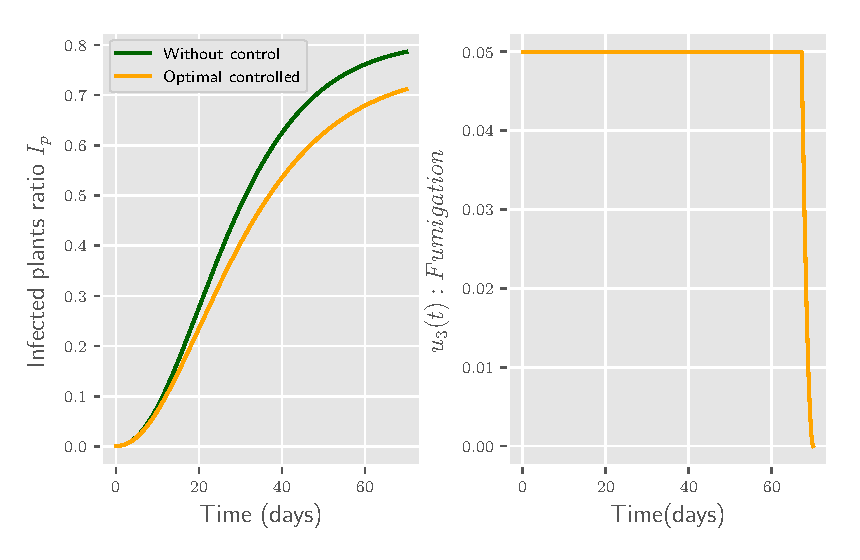
\includegraphics[scale=0.5]{Feathergraphics/figure_1_tomato_one_control.eps}
		\end{figure}	
	\end{frame}
	
	\begin{frame}
		\frametitle{Case with two controls}
		\begin{figure}
			\centering	
			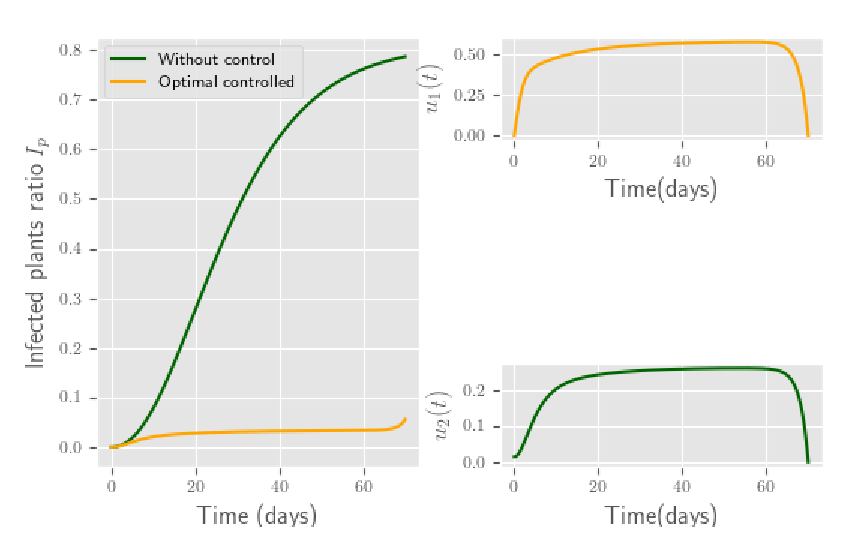
\includegraphics[scale=0.5]{Feathergraphics/two_control_simulation_2.eps}
		\end{figure}	
	\end{frame}
	
	\begin{frame}
		\begin{figure}
			\frametitle{Case with three controls}
			\centering	
			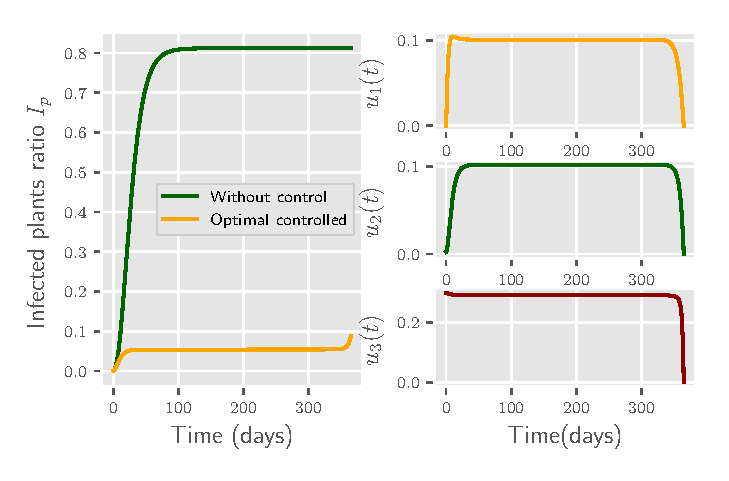
\includegraphics[scale=0.5]{Feathergraphics/three_controls_simulation_1.eps}
		\end{figure}	
	\end{frame}

\end{document}